% ============================================================
%  Milestone 1 report
%  T1: Behavioral Anomaly Detection in Agentic Tool-Use Sequences
%  Compile with pdfLaTeX + BibTeX (Overleaf default).
% ============================================================
\documentclass[11pt,a4paper]{article}

% ---------- Fill these in ----------
\newcommand{\studentname}{Alyasar Jabbarli}
\newcommand{\studentid}{Neptun code: I79D5N}
\newcommand{\supervisor}{Supervisor: Oumaima Araar}
\newcommand{\course}{Data Science Lab --- ELTE Faculty of Informatics}
% -----------------------------------

\usepackage[utf8]{inputenc}
\usepackage[T1]{fontenc}
\IfFileExists{lmodern.sty}{\usepackage{lmodern}\usepackage{microtype}}{\usepackage[expansion=false]{microtype}}
\usepackage[margin=2.5cm]{geometry}
\usepackage{amsmath,amssymb}
\usepackage{graphicx}
\usepackage{booktabs}
\usepackage{tabularx}
\usepackage{array}
\usepackage{enumitem}
\usepackage{xcolor}
\usepackage{tikz}
\usetikzlibrary{arrows.meta,positioning,fit,backgrounds,calc,shapes.geometric}
\usepackage[numbers,sort&compress]{natbib}
\usepackage[hidelinks]{hyperref}
\usepackage{xurl}
\usepackage{caption}
\captionsetup{font=small,labelfont=bf}

\newcolumntype{L}[1]{>{\raggedright\arraybackslash}p{#1}}
\newcolumntype{Y}{>{\raggedright\arraybackslash}X}
\setlist{itemsep=2pt,topsep=4pt}

\definecolor{agentblue}{HTML}{2F5D8C}
\definecolor{tooltan}{HTML}{B5762A}
\definecolor{memgreen}{HTML}{3C7A4B}
\definecolor{alertred}{HTML}{B03A2E}
\definecolor{soft}{HTML}{F3F5F8}

\title{\textbf{Behavioral Anomaly Detection in Agentic Tool-Use Sequences}\\[4pt]
\large Milestone 1 --- Field Overview and Project Scope}
\author{\studentname\\ \small \studentid\\ \small \supervisor\\ \small \course}
\date{\today}

\begin{document}
\maketitle

\begin{abstract}
\noindent Large language model (LLM) agents no longer only produce text: they call tools that send e-mails, move money, edit code and query databases. When such an agent is manipulated or simply goes wrong, the damage shows up first in \emph{what it does}, that is, in the sequence of tool calls it issues. This report places the project topic, behavioral anomaly detection over agentic tool-use sequences, inside its wider data science field. It introduces the building blocks of an LLM agent, surveys the threat categories that leave traces in tool-call sequences, outlines the main families of detection methods, explains what changes when the monitored entity is an autonomous agent instead of a program or a human user, motivates the problem with application domains and documented incidents, and defines the scope of the semester project.
\end{abstract}

\tableofcontents
\newpage

% ============================================================
\section{Definition of the General Field}
\label{sec:field}
% ============================================================

\subsection{The data science area: anomaly detection on discrete sequences}

The project belongs to \textbf{anomaly detection}, the data science task of finding observations that do not conform to a notion of expected behavior \citep{chandola2009anomaly}. Unlike standard classification, anomaly detection usually assumes that labelled examples of the abnormal class are rare, incomplete, or missing altogether, so most methods learn a model of \emph{normal} data and score how far new data departs from it. \citet{chandola2009anomaly} distinguish three kinds of anomaly, each of which has a direct counterpart in agent monitoring:
\begin{itemize}
  \item \textbf{Point anomalies}: a single item is unusual on its own (e.g.\ an agent calls a tool it has never used before).
  \item \textbf{Contextual anomalies}: an item is unusual only in a given context (e.g.\ \texttt{transfer\_money} is normal for a banking task but abnormal when the user only asked for a balance).
  \item \textbf{Collective anomalies}: individually normal items form an abnormal group (e.g.\ \texttt{read\_file} followed by \texttt{send\_email} to an external address, where each call alone is harmless).
\end{itemize}

More precisely, the project falls into \textbf{anomaly detection for discrete sequences}, where each data point is an ordered list of symbols drawn from a finite (or slowly growing) alphabet \citep{chandola2012discrete}. This sub-field has a long security tradition. \citet{forrest1996sense} showed that short windows of system calls issued by a Unix process form a compact ``sense of self'' that separates normal from intrusive executions, and \citet{du2017deeplog} later modelled system log events as a language with an LSTM, flagging an event as anomalous when the model did not expect it. A sequence of agent tool calls is structurally the same kind of object: an ordered trace of discrete events, each with parameters. The project therefore transfers well-studied sequence anomaly detection ideas to a new kind of monitored system.

\subsection{Application context: security of agentic AI}

An \textbf{AI agent} is a system in which an LLM repeatedly decides on an action, executes it through an external tool, observes the result, and decides again until the task is complete \citep{yao2023react,wang2024survey}. Agentic AI security studies how such systems can be attacked or can fail in harmful ways, and how to prevent, detect, and contain those outcomes. Industry frameworks now treat it as its own risk area: the OWASP Top~10 for LLM Applications lists \emph{Excessive Agency} as a dedicated risk \citep{owasp2025llmtop10,owasp2025llm06}, and the OWASP Agentic Security Initiative published a separate threat taxonomy for agents \citep{owasp2025agentic} followed by a Top~10 for agentic applications \citep{owasp2025agentictop10}.

\subsection{Building blocks of an AI agent}

Following the widely used decomposition of \citet{weng2023agents} and the survey of \citet{wang2024survey}, an LLM agent has four core components (Figure~\ref{fig:agent}):

\begin{description}[leftmargin=0pt,itemsep=3pt]
  \item[Language model (the ``brain'').] An LLM interprets the user's goal, reasons about the current state, and emits the next action as structured text, typically a tool name with JSON arguments. Because generation is probabilistic, the same request can produce different but equally valid action sequences.
  \item[Tools.] External functions the agent can invoke: web search, e-mail, file systems, code execution, databases, payment APIs, and so on. Models can learn when and how to call such APIs \citep{schick2023toolformer}, and tools are increasingly exposed through standard interfaces such as the Model Context Protocol (MCP). Tools are the agent's only way of acting on the world, which is why the tool-call stream is the natural place to observe its behavior.
  \item[Memory.] \emph{Short-term} memory is the context window holding the current conversation, previous actions, and tool outputs. \emph{Long-term} memory stores information across sessions, often in a vector database queried by retrieval-augmented generation (RAG) \citep{weng2023agents}.
  \item[Planning.] The agent decomposes a goal into sub-steps and adapts the plan to new observations. The ReAct pattern interleaves a free-text reasoning step (``thought'') with each action and observation \citep{yao2023react}; other designs produce a full plan first and then execute it.
\end{description}

\begin{figure}[t]
\centering
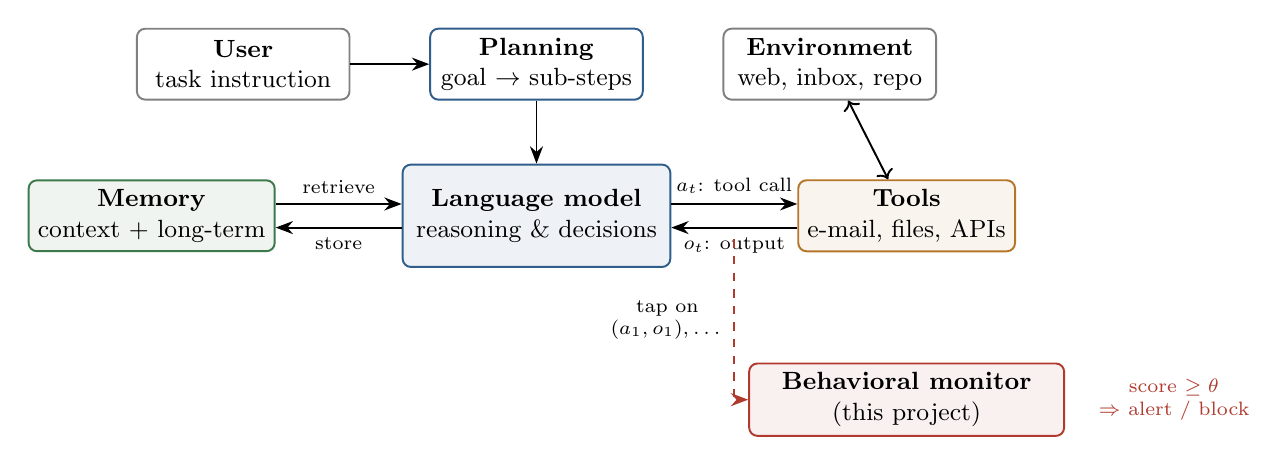
\begin{tikzpicture}[
  node distance=8mm and 10mm,
  box/.style={draw, rounded corners=3pt, minimum width=27mm, minimum height=9mm, align=center, font=\small, fill=white, line width=0.7pt},
  arr/.style={-{Stealth[length=2.2mm]}, line width=0.7pt},
  lab/.style={font=\scriptsize, align=center}
]
\node[box, draw=agentblue, fill=agentblue!8, minimum width=34mm, minimum height=13mm] (llm) {\textbf{Language model}\\ reasoning \& decisions};
\node[box, draw=agentblue, above=of llm] (plan) {\textbf{Planning}\\ goal $\rightarrow$ sub-steps};
\node[box, draw=memgreen, fill=memgreen!8, left=16mm of llm] (mem) {\textbf{Memory}\\ context + long-term};
\node[box, draw=tooltan, fill=tooltan!8, right=16mm of llm] (tools) {\textbf{Tools}\\ e-mail, files, APIs};
\node[box, left=of plan, draw=gray] (user) {\textbf{User}\\ task instruction};
\node[box, right=of plan, draw=gray] (env) {\textbf{Environment}\\ web, inbox, repo};
\draw[arr] (user) -- (plan);
\draw[arr] (plan) -- (llm);
\draw[arr, transform canvas={yshift=1.5mm}] (mem) -- node[lab, above]{retrieve} (llm);
\draw[arr, transform canvas={yshift=-1.5mm}] (llm) -- node[lab, below]{store} (mem);
\draw[arr, transform canvas={yshift=1.5mm}] (llm) -- node[lab, above]{$a_t$: tool call} (tools);
\draw[arr, transform canvas={yshift=-1.5mm}] (tools) -- node[lab, below]{$o_t$: output} (llm);
\draw[arr, <->] (tools) -- (env);
% monitor
\node[box, draw=alertred, fill=alertred!7, below=14mm of tools, minimum width=40mm] (mon) {\textbf{Behavioral monitor}\\ (this project)};
\draw[arr, dashed, draw=alertred] ($(llm.east)!0.5!(tools.west)+(0,-3mm)$) |- node[lab, pos=0.25, left]{tap on\\$(a_1,o_1),\dots$} (mon.west);
\node[lab, right=3mm of mon, text=alertred] {score $\geq \theta$\\ $\Rightarrow$ alert / block};
\end{tikzpicture}
\caption{Building blocks of an LLM agent and where a behavioral monitor sits. The monitor passively observes the stream of tool calls $a_t$ and outputs $o_t$. Figure made by the author, based on the component decomposition in \citep{weng2023agents,wang2024survey}.}
\label{fig:agent}
\end{figure}

\subsection{Key terms used in this project}

Table~\ref{tab:terms} fixes the vocabulary used in the rest of the report and the project.

\begin{table}[h]
\centering
\small
\begin{tabularx}{\linewidth}{L{3.3cm}Y}
\toprule
\textbf{Term} & \textbf{Meaning in this project} \\
\midrule
Tool call / action $a_t$ & One invocation $a_t = (\text{tool name}, \text{arguments})$ issued by the agent at step $t$. \\
Observation $o_t$ & The tool's returned output, which enters the agent's context. \\
Trajectory / trace $\tau$ & The full record of one task: $\tau = \big(u, (a_1,o_1), \dots, (a_T,o_T)\big)$, where $u$ is the user instruction. Its length $T$ varies between tasks. \\
Tool-use sequence & The projection of $\tau$ onto actions only, $(a_1,\dots,a_T)$; in its simplest form, just the sequence of tool names. \\
Workflow & A family of tasks of the same kind (e.g.\ ``summarise inbox'', ``book a trip'') that share a typical set of tool patterns. \\
Behavioral baseline & A learned model of normal tool-use sequences for a workflow or agent. \\
Anomaly score $s(\cdot)$ & A real number measuring how far a (partial) trajectory deviates from the baseline; an alert is raised when $s \geq \theta$. \\
Online / prefix detection & Scoring the partial trajectory $\tau_{1:t}$ after each step, so that an alert can fire \emph{before} a harmful action executes. \\
False positive rate (FPR) & Share of benign trajectories wrongly flagged; it must stay low for a monitor to be usable. \\
Attack success rate (ASR) & Share of attack attempts in which the attacker's goal is achieved; the standard metric in agent security benchmarks. \\
Indirect prompt injection & Malicious instructions hidden in data the agent reads through a tool, rather than typed by the user \citep{greshake2023indirect}. \\
\bottomrule
\end{tabularx}
\caption{Key terms.}
\label{tab:terms}
\end{table}

% ============================================================
\section{Types of Threats Related to the Topic}
\label{sec:threats}
% ============================================================

The project is concerned with threats that \emph{change what the agent does}, because those are the ones visible in a tool-call trace. Following the component view of Section~\ref{sec:field} and the OWASP agentic taxonomy \citep{owasp2025agentic}, they can be grouped by where the harmful influence enters the agent. Table~\ref{tab:threats} summarises how each category typically shows up in a tool-use sequence.

\paragraph{1. Indirect prompt injection and goal hijacking.} The attacker plants instructions in content the agent will read through a tool, such as a web page, e-mail, document, or code issue. The LLM cannot reliably separate data from instructions, so it may follow the planted text and abandon the user's goal \citep{greshake2023indirect}. \emph{Example:} a user asks the agent to summarise today's e-mails; one message contains hidden text telling the agent to forward the user's latest invoice to an outside address. The resulting trace contains an unexpected \texttt{send\_email} after \texttt{read\_inbox}. Benchmarks show this is common: on InjecAgent, a ReAct-prompted GPT-4 agent followed injected instructions in 24\% of cases, and adding a ``hacking prompt'' to the injection nearly doubled that rate \citep{zhan2024injecagent}.

\paragraph{2. Direct prompt injection and malicious use.} Here the user (or whoever controls the user channel) is the attacker and asks the agent to perform harmful actions, often wrapped in jailbreak phrasing. \emph{Example:} a request disguised as a ``security audit'' that makes a DevOps agent disable logging and create a new admin account. Agent Security Bench evaluates such direct attacks alongside indirect ones \citep{zhang2025asb}.

\paragraph{3. Memory and knowledge-base poisoning.} The attacker inserts malicious records into the agent's long-term memory or RAG store, so that harmful behavior is triggered later, possibly in another session. \emph{Example:} AgentPoison inserted a small number of poisoned demonstrations into the memory of an autonomous-driving agent so that queries containing a trigger led to a dangerous ``sudden stop'' action; with a poisoning ratio below 0.1\%, it reached an average attack success rate of at least 80\% while benign performance dropped by less than 1\% \citep{chen2024agentpoison}.

\paragraph{4. Tool poisoning and supply-chain compromise.} The attack targets the tools themselves: a third-party tool or MCP server ships a description or implementation that carries hidden instructions or malicious logic. Tool poisoning is a special case of indirect injection that rides on the tool's metadata rather than its output \citep{wallarm2025mcp}. \emph{Example:} a harmless-looking ``add numbers'' tool whose description instructs the agent to first read a local configuration file and pass its contents as an argument; the trace shows a file read that has nothing to do with the task.

\paragraph{5. Tool misuse and excessive agency.} The agent uses a tool it is allowed to use, but in a way nobody intended, typically because it was given more functionality, permissions, or autonomy than the task needs \citep{owasp2025llm06}. \emph{Example:} an agent with read--write database credentials asked to ``clean up test data'' issues a \texttt{DROP TABLE} on production.

\paragraph{6. Data exfiltration through tool chains.} A combination of tool calls moves private data to a destination the attacker controls. Each call may be authorised, but the \emph{sequence} forms what Invariant Labs called a ``toxic agent flow'' \citep{invariant2025github}. \emph{Example:} in the GitHub MCP case, a malicious issue in a public repository hijacked the user's agent and made it leak data from the user's private repositories \citep{invariant2025github}. Microsoft's EchoLeak vulnerability (CVE-2025-32711, CVSS 9.3) let an attacker's e-mail cause Microsoft 365 Copilot to leak internal data without any user click \citep{thn2025echoleak}.

\paragraph{7. Non-adversarial unsafe behavior.} Not every anomaly is an attack. Agents misunderstand ambiguous instructions, loop, hallucinate tool results, or take destructive shortcuts. ToolEmu found that even the safest agent it evaluated still exhibited potentially severe failures 23.9\% of the time \citep{ruan2024toolemu}. \emph{Example:} in July 2025 a coding agent deleted a production database during an explicit code freeze \citep{eweek2025replit,aiid2025replit}.

\paragraph{8. Covert sabotage by a misaligned agent.} The agent itself pursues a hidden objective while appearing to complete the main task. \emph{Example:} SHADE-Arena pairs benign main tasks with hidden harmful side tasks in realistic tool environments (e.g.\ a bank-transfer task in which money is quietly sent to the wrong account) and measures whether an LLM monitor can tell sabotaged transcripts apart; the best monitor reached an AUC of 0.87 \citep{kutasov2025shade}. These traces are especially hard because the harmful steps are few and buried among many legitimate ones.

\paragraph{How the categories differ.} Categories 1--4 differ by \emph{entry point} (tool output, user prompt, memory, tool definition), while categories 5--8 describe \emph{what goes wrong} regardless of how it started. Only category 7 is unintentional. For a behavioral monitor the distinction matters less than one might expect: all eight categories end with the agent executing an action, or an ordering of actions, that is unusual for the task. This is precisely what makes behavior a useful common signal across very different root causes.

\begin{table}[t]
\centering
\small
\begin{tabularx}{\linewidth}{L{3.3cm}L{2.6cm}Y}
\toprule
\textbf{Threat category} & \textbf{Entry point} & \textbf{Typical signature in a tool-use sequence} \\
\midrule
Indirect prompt injection & Tool output & Off-task call right after reading untrusted content; new recipient or destination \\
Direct injection / misuse & User prompt & Sensitive tools used from the first steps; unusual argument values \\
Memory / RAG poisoning & Long-term memory & Abnormal action appears after a retrieval step, often reproducibly for a trigger \\
Tool poisoning & Tool definition & Calls to unrelated tools (e.g.\ file reads) before or inside a benign tool's use \\
Tool misuse / excessive agency & Permissions & Rare, high-impact operations (delete, transfer, privilege change) \\
Data exfiltration & Combination & Read of private data followed by a write to an external sink (collective anomaly) \\
Non-adversarial failure & Model error & Loops, repeated failing calls, destructive shortcuts, abnormally long traces \\
Covert sabotage & Agent itself & Few extra steps hidden in a long, mostly normal trajectory \\
\bottomrule
\end{tabularx}
\caption{Threat categories and how they surface in tool-call traces. Categories adapted from \citep{owasp2025agentic,zhang2025asb}; signatures are the author's synthesis.}
\label{tab:threats}
\end{table}

% ============================================================
\section{Types of Detection Methods}
\label{sec:methods}
% ============================================================

Detection methods for agent misbehavior can be grouped into families according to \emph{what they inspect} (inputs, reasoning, or actions) and \emph{how they decide} (rules, statistics, learned models, or another LLM). The families below are ordered roughly from simplest to most expressive. Table~\ref{tab:methods} summarises their trade-offs.

\paragraph{A. Rule-, policy- and specification-based methods.} Security engineers write explicit constraints: allow-lists of tools per task, forbidden orderings (``never \texttt{send\_email} after \texttt{read\_secret}''), rate limits, or approval gates for high-impact operations. A stronger variant restricts information flow by construction: CaMeL extracts the control and data flow from the trusted user query so that untrusted tool outputs cannot change which tools are called, and it solved 77\% of AgentDojo tasks with provable security versus 84\% for an undefended system \citep{debenedetti2025camel}. \emph{Strengths:} precise, interpretable, predictable cost. \emph{Weaknesses:} rules must be written per workflow, do not cover unforeseen attacks, and become brittle as tools and tasks change.

\paragraph{B. Statistical sequence models.} Normal behavior is captured by the statistics of short subsequences. The classic approach stores all length-$k$ windows (n-grams) seen in normal traces and flags unseen ones \citep{forrest1996sense}; probabilistic versions use Markov chains or hidden Markov models and flag low-likelihood transitions \citep{chandola2012discrete}. \emph{Strengths:} simple, fast, need only normal data, easy to explain (``this transition was never seen''). \emph{Weaknesses:} limited memory of long-range context, sensitive to the choice of $k$, and they ignore tool arguments unless these are discretised.

\paragraph{C. Classical machine learning on engineered features.} Each trajectory is turned into a fixed-length feature vector (tool counts, transition frequencies, trace length, argument statistics) and scored with a general-purpose detector such as one-class SVM \citep{scholkopf2001oneclass} or Isolation Forest \citep{liu2008isolation}; supervised classifiers can be used when labelled attacks exist. \emph{Strengths:} mature tooling, handle variable length through aggregation, cheap at inference. \emph{Weaknesses:} the aggregation discards order, so collective anomalies can be missed, and results depend heavily on feature design.

\paragraph{D. Deep sequence models.} Recurrent networks such as LSTMs \citep{hochreiter1997lstm}, autoencoders, and transformers learn the structure of normal sequences directly. A common scheme predicts the next event and raises an alarm when the observed event is not among the most likely ones, as DeepLog does for system logs \citep{du2017deeplog}. LogBERT replaces the recurrent network with a BERT-style transformer that is trained on normal log sequences through self-supervised tasks and flags sequences whose patterns deviate from them \citep{guo2021logbert}; another family reconstructs the sequence and uses reconstruction error as the score. In the agent setting, Trajectory Guard trains a recurrent autoencoder on tool-call trajectories and reports F1 between 0.88 and 0.94 on balanced test sets at about 32\,ms per trajectory \citep{advani2026trajectoryguard}. \emph{Strengths:} capture long-range order and variable length natively, can embed arguments. \emph{Weaknesses:} need large amounts of normal data, are harder to interpret, and can be fooled by attacks that look statistically normal.

\paragraph{E. Graph- and provenance-based methods.} Traces are converted into graphs whose nodes are tool calls (or agents) and whose edges encode order and data dependencies, so that the method can ask which output flowed into which input. TraceAegis learns hierarchical templates of normal execution units from agent traces and checks new traces against them, reaching a best F1 score of 0.965 on its clinical triage (healthcare) scenario and 0.936 on its procurement scenario \citep{liu2025traceaegis}; SentinelAgent builds execution graphs of multi-agent systems and applies anomaly checks over nodes and edges \citep{he2025sentinelagent}. \emph{Strengths:} model data flow, which is exactly what exfiltration exploits; structured explanations. \emph{Weaknesses:} need richer logging (data provenance), and graph construction adds engineering cost.

\paragraph{F. LLM-based monitors and judges.} A second LLM reads the trajectory, or the agent's reasoning, and judges whether it still serves the user's goal. LlamaFirewall's AlignmentCheck audits the agent's chain of thought for signs of goal hijacking \citep{chennabasappa2025llamafirewall}; SHADE-Arena uses LLM monitors to rate how suspicious a transcript is \citep{kutasov2025shade}; TrajAD fine-tunes a verifier LLM to flag a faulty trajectory and locate its first wrong step \citep{liu2026trajad}. \emph{Strengths:} understand semantics and task context with little or no training data. \emph{Weaknesses:} expensive and slow per step, themselves vulnerable to injection, and still imperfect on subtle cases (best AUC 0.87 in SHADE-Arena \citep{kutasov2025shade}).

\paragraph{G. Input-level injection detectors (contrast family).} Classifiers that scan prompts or tool outputs for injected instructions before they reach the agent. They are not behavioral, but they are the most common deployed baseline. In AgentDojo, adding such a detector lowered the attack success rate to 8\% \citep{debenedetti2024agentdojo}. Their blind spot is that they look at text, not consequences, so poisoning, misuse, and non-adversarial failures pass unnoticed; this motivates complementing them with behavioral monitoring.

\paragraph{Learning regimes.} Orthogonal to the families above, methods differ by supervision: \emph{unsupervised} (no labels), \emph{semi-supervised / one-class} (only normal data, the most common setting in anomaly detection \citep{chandola2009anomaly}), and \emph{supervised} (labelled attacks, which risks overfitting to known attack types). The project focuses on the one-class setting because normal traces are cheap to collect while attacks are open-ended.

\begin{table}[t]
\centering
\small
\begin{tabularx}{\linewidth}{L{2.7cm}L{2.4cm}YY}
\toprule
\textbf{Family} & \textbf{Data needed} & \textbf{Main strengths} & \textbf{Main weaknesses} \\
\midrule
A. Rules / policies & Expert knowledge & Precise, explainable, cheap & Manual, brittle, misses novel attacks \\
B. Statistical sequence & Normal traces & Simple, fast, interpretable & Short memory, ignores arguments \\
C. Classical ML & Normal (or labelled) traces & Mature tools, handles variable length & Loses order, feature-dependent \\
D. Deep sequence & Many normal traces & Long-range order, embeds arguments & Data-hungry, opaque \\
E. Graph / provenance & Traces with data flow & Captures data flow and exfiltration & Heavier logging and engineering \\
F. LLM monitor & Few or none & Semantic, task-aware & Costly, slow, injectable itself \\
G. Input detectors & Labelled prompts & Blocks known injections early & Blind to behavior and non-text threats \\
\bottomrule
\end{tabularx}
\caption{Families of detection methods. Summary by the author; representative results are cited in the text.}
\label{tab:methods}
\end{table}

\subsection{Key literature for the project}
\label{sec:keypapers}
Table~\ref{tab:keypapers} lists the ten papers that will be reviewed in depth in Milestone~2. The two Chandola surveys \citep{chandola2009anomaly,chandola2012discrete} are used as background for the field and are not part of the ten. InjecAgent \citep{zhan2024injecagent} is cited for its threat statistics but is not selected as a trace source: it overlaps with AgentDojo and ASB, and its attack cases are mostly single-step, which gives little sequence structure to learn from.

\begin{table}[ht]
\centering
\small
\begin{tabularx}{\linewidth}{L{2.3cm}L{5.4cm}Y}
\toprule
\textbf{Group} & \textbf{Paper} & \textbf{Role in the project} \\
\midrule
Detection methods & Forrest et al.\ 1996 \citep{forrest1996sense} & n-gram baseline on system-call sequences (family B) \\[3pt]
 & DeepLog, Du et al.\ 2017 \citep{du2017deeplog} & LSTM next-event baseline (family D) \\[3pt]
 & LogBERT, Guo et al.\ 2021 \citep{guo2021logbert} & Transformer-based sequence detector (family D) \\[3pt]
 & TraceAegis, Liu et al.\ 2025 \citep{liu2025traceaegis} & Anomaly detection over agent tool-call traces (family E) \\[3pt]
 & LlamaFirewall, Chennabasappa et al.\ 2025 \citep{chennabasappa2025llamafirewall} & LLM-based monitor of agent reasoning (family F) \\[3pt]
 & SHADE-Arena, Kutasov et al.\ 2025 \citep{kutasov2025shade} & LLM monitors on long sabotage transcripts (family F) \\
\midrule
Attacks and benchmarks & AgentDojo, Debenedetti et al.\ 2024 \citep{debenedetti2024agentdojo} & Main candidate trace source (e-mail, banking, travel) \\[3pt]
 & ASB, Zhang et al.\ 2025 \citep{zhang2025asb} & Second trace source; 10 domains, 400+ tools \\[3pt]
 & AgentPoison, Chen et al.\ 2024 \citep{chen2024agentpoison} & Threat visible only through behavior \\
\midrule
Prevention & CaMeL, Debenedetti et al.\ 2025 \citep{debenedetti2025camel} & Design-level alternative; motivates detection \\
\bottomrule
\end{tabularx}
\caption{Papers selected for in-depth review, grouped by role.}
\label{tab:keypapers}
\end{table}

% ============================================================
\section{Overview of the Specific Topic}
\label{sec:topic}
% ============================================================

\subsection{Problem statement}

Given a corpus of trajectories produced by an agent while performing legitimate tasks, the goal is to learn a scoring function $s$ such that, for a new (possibly partial) trajectory $\tau_{1:t}$, the score $s(\tau_{1:t})$ is low when the behavior is consistent with normal behavior for that kind of task and high when it is not. A trajectory is flagged when $s(\tau_{1:t}) \geq \theta$, where the threshold $\theta$ trades detection rate against false alarms. Figure~\ref{fig:example} shows the intuition on a simple e-mail workflow.

\begin{figure}[t]
\centering
\resizebox{\linewidth}{!}{%
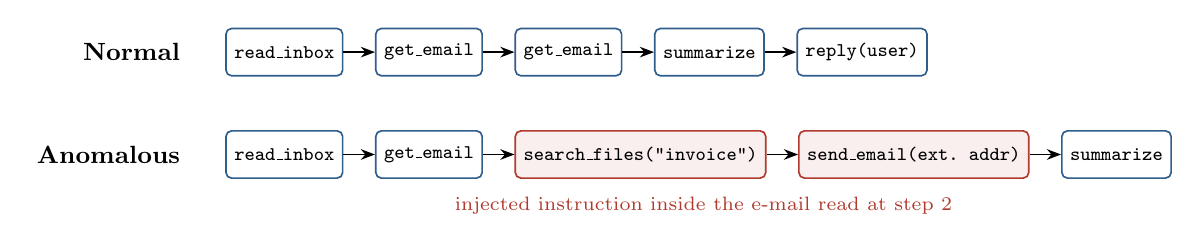
\begin{tikzpicture}[
  call/.style={draw, rounded corners=2pt, font=\scriptsize\ttfamily, minimum height=6mm, inner xsep=3pt, fill=white, line width=0.6pt},
  arr/.style={-{Stealth[length=1.8mm]}, line width=0.6pt},
  lab/.style={font=\small\bfseries, anchor=east}
]
\node[lab] at (-0.3,0) {Normal};
\node[call, draw=agentblue] (n1) at (0.9,0) {read\_inbox};
\node[call, draw=agentblue, right=4mm of n1] (n2) {get\_email};
\node[call, draw=agentblue, right=4mm of n2] (n3) {get\_email};
\node[call, draw=agentblue, right=4mm of n3] (n4) {summarize};
\node[call, draw=agentblue, right=4mm of n4] (n5) {reply(user)};
\foreach \a/\b in {n1/n2,n2/n3,n3/n4,n4/n5} \draw[arr] (\a) -- (\b);

\node[lab] at (-0.3,-1.3) {Anomalous};
\node[call, draw=agentblue] (a1) at (0.9,-1.3) {read\_inbox};
\node[call, draw=agentblue, right=4mm of a1] (a2) {get\_email};
\node[call, draw=alertred, fill=alertred!8, right=4mm of a2] (a3) {search\_files("invoice")};
\node[call, draw=alertred, fill=alertred!8, right=4mm of a3] (a4) {send\_email(ext.\ addr)};
\node[call, draw=agentblue, right=4mm of a4] (a5) {summarize};
\foreach \a/\b in {a1/a2,a2/a3,a3/a4,a4/a5} \draw[arr] (\a) -- (\b);
\node[font=\scriptsize, text=alertred, below=1mm of a3, xshift=8mm] {injected instruction inside the e-mail read at step 2};
\end{tikzpicture}}
\caption{Illustrative tool-use sequences for the task ``summarise my unread e-mails''. The anomalous trace contains individually plausible calls in an order and with arguments that never occur in normal traces for this workflow (a collective and contextual anomaly). Figure made by the author.}
\label{fig:example}
\end{figure}

\subsection{What changes when the monitored system is an autonomous agent}

Behavioral anomaly detection is not new: it has been applied to programs through system calls \citep{forrest1996sense} and logs \citep{du2017deeplog}, and to human users through behavior analytics. An LLM agent differs from both in ways that shape the whole project.

\paragraph{Compared with a traditional application.}
\begin{itemize}
  \item \textbf{Control flow is generated, not compiled.} A program's possible call sequences are fixed by its code, so normal behavior is a fairly tight set. An agent's control flow is produced by the LLM at run time, so the same task can yield several valid sequences. ``Normal'' becomes a \emph{distribution} over sequences rather than a set of allowed paths, which raises the false-alarm risk.
  \item \textbf{Normality depends on the task.} A program performs the same function in each run; an agent performs whatever the user asked. The same trace can be normal for one instruction and alarming for another, so detection is inherently contextual and should be conditioned on the task or workflow.
  \item \textbf{Arguments carry the meaning.} \texttt{send\_email} is harmless or harmful depending on the recipient and content. Symbol-only models that work for system calls must be extended with argument and data-flow features.
  \item \textbf{The attacker acts through data, mid-execution.} In classic intrusion detection the attacker usually exploits a code flaw. Here the attacker only needs to place text where the agent will read it, and the hijack happens inside a single legitimate session, using the agent's legitimate credentials \citep{greshake2023indirect,invariant2025github}.
  \item \textbf{The tool vocabulary is open.} New tools and MCP servers can be added at any time, so the alphabet of the sequence is not fixed and unseen symbols are expected rather than exceptional.
\end{itemize}

\paragraph{Compared with a human user.}
\begin{itemize}
  \item \textbf{Speed and scale.} An agent can issue many actions in seconds without the natural pauses in which a human, or a reviewer, would notice a mistake. Detection must therefore be online and fast enough to stop an action before it executes.
  \item \textbf{The agent can be steered by anyone whose text it reads.} A human employee is rarely re-programmed by a sentence inside an e-mail; an agent can be. The insider-threat model of user behavior analytics shifts from ``a malicious person'' to ``a well-meaning system that was hijacked''.
  \item \textbf{Reasoning traces exist but are not trustworthy.} Agents often expose their intermediate reasoning, which offers an extra signal unavailable for humans \citep{chennabasappa2025llamafirewall}. However, this text may itself be manipulated, and agents perform sabotage better when part of their reasoning is hidden from the monitor \citep{kutasov2025shade}. This project therefore relies primarily on actions, which are harder to fake because they have real effects.
  \item \textbf{Behavior shifts with every model or prompt update.} A human's habits drift slowly; an agent's behavior can change overnight when its underlying model, system prompt, or toolset is updated. Baselines need to be re-learned or adapted, and distribution shift must be part of the evaluation.
\end{itemize}

\paragraph{Resulting challenges for the project.} These differences map directly onto the challenges in the topic description: (i)~defining normal tool-use patterns per task family; (ii)~detecting abnormal orderings and arguments rather than only unseen tools; (iii)~handling variable-length, branching sequences; and (iv)~keeping false alarms low despite legitimate variability.

% ============================================================
\section{Motivation and Application Domains}
\label{sec:motivation}
% ============================================================

\subsection{Why the problem matters}

\paragraph{Adoption is growing fast.} Gartner predicts that 33\% of enterprise software applications will include agentic AI by 2028, up from less than 1\% in 2024, and that at least 15\% of day-to-day work decisions will be made autonomously by agents by then \citep{gartner2025agentic}. The same report also expects over 40\% of agentic AI projects to be cancelled by the end of 2027, citing among other reasons inadequate risk controls \citep{gartner2025agentic}.

\paragraph{Agents remain highly vulnerable.} Across 13 LLM backbones, Agent Security Bench measured a highest average attack success rate of 84.30\%, with current defenses showing limited effectiveness \citep{zhang2025asb}. On AgentDojo, state-of-the-art models completed fewer than 66\% of tasks even without attacks, and existing prompt injection attacks still broke some security properties \citep{debenedetti2024agentdojo}.

\paragraph{Prevention alone is not enough.} Design-level defenses such as CaMeL show that strong guarantees are possible, but at a cost in utility (77\% vs.\ 84\% task success in AgentDojo \citep{debenedetti2025camel}). Input detectors miss threats that are not visible as suspicious text \citep{debenedetti2024agentdojo}. Defense in depth therefore needs a layer that watches what the agent actually does, regardless of why it is doing it. Behavioral monitoring is that layer, and it also catches non-adversarial failures, which input filters by construction cannot.

\paragraph{Real incidents already exist.} EchoLeak showed a zero-click data leak from an enterprise assistant \citep{thn2025echoleak}; the GitHub MCP case showed private source code exfiltrated through an ordinary agent session \citep{invariant2025github}; and a coding agent's deletion of a production database showed that harm does not require an attacker \citep{eweek2025replit,aiid2025replit}. In each case, the harmful step was a tool call that was out of character for the task the user had given.

\subsection{Application domains}

Behavioral anomaly detection over tool calls is relevant wherever agents act with real permissions:

\begin{description}[leftmargin=0pt,itemsep=3pt]
  \item[Enterprise productivity and e-mail assistants.] Agents that read and write mail, calendars, and shared documents are exposed to injected content in every incoming message; EchoLeak is a concrete example \citep{thn2025echoleak}. AgentDojo's workspace tasks model this setting \citep{debenedetti2024agentdojo}.
  \item[Software engineering and DevOps.] Coding agents run shell commands, edit repositories, and access CI/CD secrets. Examples include the GitHub MCP exfiltration \citep{invariant2025github} and the production database deletion \citep{eweek2025replit}.
  \item[Banking and finance.] Agents that read statements and initiate payments make fraudulent transfers a direct risk; AgentDojo includes an e-banking environment \citep{debenedetti2024agentdojo} and ASB includes finance and investment scenarios \citep{zhang2025asb}.
  \item[Healthcare.] Clinical agents query electronic health records. AgentPoison attacked a healthcare EHR agent \citep{chen2024agentpoison}, and TraceAegis evaluates a clinical triage agent \citep{liu2025traceaegis}.
  \item[E-commerce, travel, and customer service.] Booking and shopping agents handle payments and personal data while reading untrusted web content and reviews; ASB covers e-commerce \citep{zhang2025asb} and AgentDojo covers travel booking \citep{debenedetti2024agentdojo}.
  \item[Cyber-physical and autonomous systems.] When an agent's actions drive physical systems, an abnormal action can be dangerous in itself, as in AgentPoison's ``sudden stop'' attack on a driving agent \citep{chen2024agentpoison}; ASB also includes an autonomous driving scenario \citep{zhang2025asb}.
\end{description}

% ============================================================
\section{Scope}
\label{sec:scope}
% ============================================================

\subsection{In scope}
\begin{itemize}
  \item \textbf{Single-agent tool-call traces.} The unit of analysis is one agent completing one task. This keeps the problem well defined and matches the format of most public agent security benchmarks.
  \item \textbf{Action-level behavioral signals.} Tool names, their order, and coarse argument features (e.g.\ argument type, whether a recipient or URL is internal or external, whether a value comes from untrusted content). Actions are the most robust signal because they have real effects and are always logged.
  \item \textbf{Semi-supervised (one-class) detection,} with labelled attacks used only for evaluation. Normal traces are cheap to generate, while the space of attacks is open-ended; training only on normal data avoids overfitting to known attacks.
  \item \textbf{Both whole-trace and prefix (online) scoring,} so that the project can measure how early in a trajectory an anomaly is detected, which determines whether a harmful action could be blocked in time.
  \item \textbf{Several workflows,} to test how well a baseline transfers across task types and how false alarms behave when legitimate variability differs between workflows, as required by the project objectives.
  \item \textbf{Comparison of method families} B, C, and D from Section~\ref{sec:methods}, with simple rules (A) as a baseline and an LLM monitor (F) as an optional reference point if budget allows.
  \item \textbf{Evaluation} with detection metrics (precision, recall, F1, ROC-AUC), FPR at fixed recall, and detection delay (number of steps before the first harmful action).
\end{itemize}

\subsection{Out of scope}
\begin{itemize}
  \item \textbf{Preventing attacks or hardening the agent} (prompt design, fine-tuning, architectural isolation such as CaMeL). The project detects; it does not redesign the agent. Prevention is a different research question and is studied extensively elsewhere \citep{debenedetti2025camel}.
  \item \textbf{Input-level prompt-injection classification.} Text classifiers on prompts are a separate topic; here they serve only as a contrast.
  \item \textbf{Multi-agent collusion and agent-to-agent protocols.} Multi-agent systems add inter-agent graphs and new threat types \citep{he2025sentinelagent}; they would roughly double the problem size. They may be revisited as an extension.
  \item \textbf{Model internals} such as attention weights or hidden activations. Requiring white-box access would exclude closed commercial models, which power many deployed agents; the monitor should work from externally observable logs.
  \item \textbf{Judging the content quality or factual accuracy of answers,} which is a hallucination or evaluation problem rather than a behavioral one.
  \item \textbf{Live deployment on real user data.} Experiments will use public benchmarks or synthetic traces, avoiding privacy and safety issues of monitoring real users.
\end{itemize}

\subsection{Next steps}
The next milestones will review representative papers in depth, select trace sources (AgentDojo and ASB are the main candidates, see Table~\ref{tab:keypapers}), design the sequence representation, and implement the first baselines.

% ============================================================
\bibliographystyle{plainnat}
\bibliography{references}

\end{document}
